\iffalse
\documentclass[12pt]{article}
\usepackage{graphicx}
\usepackage[none]{hyphenat}
\usepackage{graphicx}
\usepackage{listings}
\usepackage[english]{babel}
\usepackage{graphicx}
\usepackage{caption} 
\usepackage{booktabs}
\usepackage{array}
\usepackage{amssymb} % for \because
\usepackage{amsmath}   % for having text in math mode
\usepackage{extarrows} % for Row operations arrows
\usepackage{listings}
\usepackage[utf8]{inputenc}
\lstset{
  frame=single,
  breaklines=true
}
\usepackage{hyperref}
  
%Following 2 lines were added to remove the blank page at the beginning
\usepackage{atbegshi}% http://ctan.org/pkg/atbegshi
\AtBeginDocument{\AtBeginShipoutNext{\AtBeginShipoutDiscard}}


%New macro definitions
\newcommand{\mydet}[1]{\ensuremath{\begin{vmatrix}#1\end{vmatrix}}}
\providecommand{\brak}[1]{\ensuremath{\left(#1\right)}}
\newcommand{\solution}{\noindent \textbf{Solution: }}
\newcommand{\myvec}[1]{\ensuremath{\begin{pmatrix}#1\end{pmatrix}}}
\providecommand{\norm}[1]{\left\lVert#1\right\rVert}
\providecommand{\abs}[1]{\left\vert#1\right\vert}
\let\vec\mathbf

\begin{document}

\begin{center}
\title{\textbf{VECTORS}}
\date{\vspace{-5ex}} %Not to print date automatically
\maketitle
\end{center}

\section{10$^{th}$ Maths - EXERCISE-7.3}

\begin{enumerate}
\item That a median of a triangle divides it into two triangles  of equal areas. verify this result for $\triangle ABC$ whose vertices are $\vec{A}(4,-6),\vec{B}(3,-2)\text{ and }\vec{C}(5,2)$.
\end{enumerate}

\section{SOLUTION}
Given points are
\begin{align}
\vec{A}=\myvec{4\\ -6} ,
\vec{B}=\myvec{3\\ -2} ,
\vec{C}=\myvec{5\\ 2}
\end{align}
\fi
The median of the triangle 
\begin{align}
\vec{D}&=\frac{\vec{B}+\vec{C}}{2}\\
&=\myvec{4\\ 0}
\end{align}
Since 
\begin{align}
	\vec{A}- \vec{B} &= \myvec{4\\ -6}-\myvec{3\\ -2}=\myvec{1\\ -4}\label{eq:10/7/3/5/7}\\
	  \vec{A}- \vec{D} &= \myvec{4\\ -6}-\myvec{4\\ 0}=\myvec{0\\ -6}\label{eq:10/7/3/5/8}
  \end{align}
 \begin{align}
  ar(ABD)&=\frac{1}{2} \norm{\brak{\vec{A}-\vec{B}}  \times 
   \brak{\vec{A}- \vec{D}}} \label{eq:10/7/3/5/6} 
   \\
&=\frac{1}{2}\mydet{1 & 0\\-4 & -6}
	       =3	
\end{align}
upon
Substituting from \eqref{eq:10/7/3/5/7} and \eqref{eq:10/7/3/5/8} in \eqref{eq:10/7/3/5/6}.
		Similarly, 
\begin{align}
	\vec{A}- \vec{C} &= \myvec{4\\ -6}-\myvec{5\\ 2}=\myvec{-1\\ -8}\label{eq:10/7/3/5/13} \\
	  \vec{A}- \vec{D} &= \myvec{4\\ -6}-\myvec{4\\ 0}=\myvec{0\\ -6}\label{eq:10/7/3/5/14} 
  \end{align}
  yielding
  \begin{align}
  ar(ACD)&=\frac{1}{2} \norm{\brak{\vec{A}-\vec{C}}  \times 
   \brak{\vec{A}- \vec{D}}} \label{eq:10/7/3/5/12}
   \\
	&=\frac{1}{2}\mydet{-1 & 0\\-8 & -6}= 3
\end{align}
upon substituting from \eqref{eq:10/7/3/5/13} and \eqref{eq:10/7/3/5/14} in \eqref{eq:10/7/3/5/12}.
Thus,
\begin{align}
ar(ABD)=ar(ACD)
\end{align}
See Fig. 
\ref{fig:10/7/3/5/}.
\begin{figure}[h!]
\centering
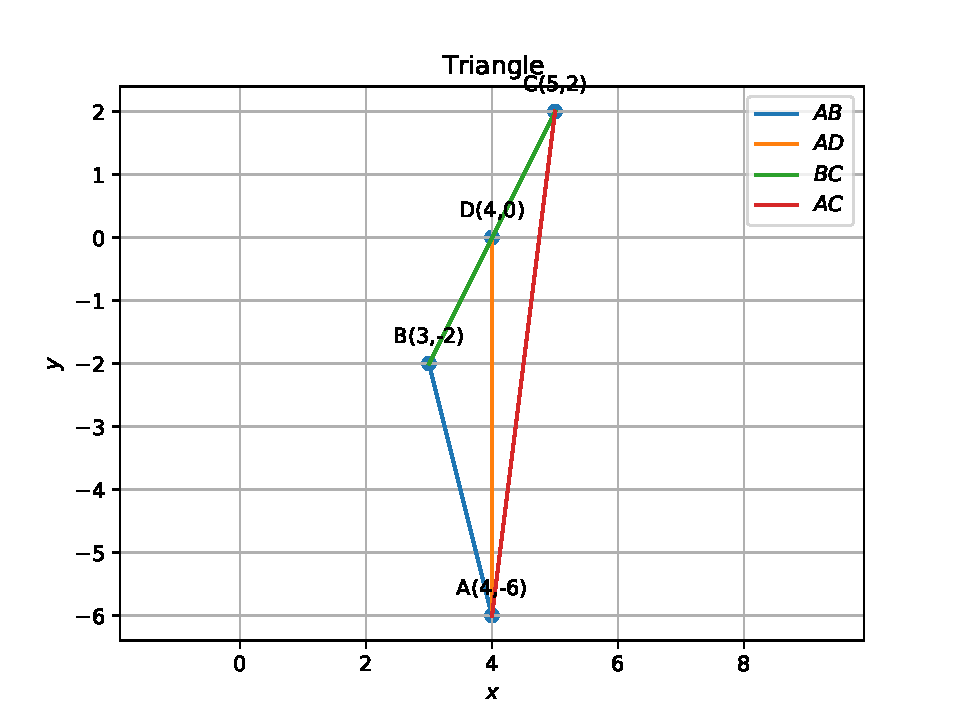
\includegraphics[width=\columnwidth]{chapters/10/7/3/5/figs/fig.pdf}
\caption{}
\label{fig:10/7/3/5/}
\end{figure} 
